\section{\sysname{}}
\label{sec:arch}

\subsection{Overview}
\label{subsec:system_overview}
%
Building upon the aforementioned principles, we propose \sysname{}, a
PIM-enabled system designed to accelerate state update and attention
operations while minimizing PIM area overhead.
%
We first focus on \sysname{} as a state update operation accelerator,
while attention operation acceleration is detailed in
Section~\ref{subsec:attention_support}.
%
Figure~\ref{fig:overview_system} provides a high-level overview of
\sysname{} system.
%

%
\niparagraph{(1) \sysname{} system.}
%
\sysname{} handles user requests in two phases: prefill and generation.
%
In the prefill phase, all operations, including state updates, run on
the GPU, as they can be restructured into compute-intensive
forms~\cite{retnet, mamba2}.
%
In the generation phase, \sysname{} offloads the state update and
attention operations to the PIM, while other operations remain on the GPU.
%
For the PIM-executed operations, \sysname{} transfers operands to PIM
registers, computes partial sums, and sends the results back to the
GPU for accumulation.
%

%
To support heterogeneous execution, \sysname{} includes a software
stack based on a prior work, HBM-PIM~\cite{hbm_pim}.
%
As in HBM-PIM~\cite{hbm_pim}, \sysname{} device driver first
allocates physically contiguous memory blocks to facilitate
efficient PIM operations.
%
Custom GPU kernels are implemented for each \sysname{} operation to
issue the necessary PIM commands and compute the addresses of the
memory regions involved in the computations.
%
To support this, the GPU programming model (e.g., CUDA) is extended
with APIs to issue \sysname{}'s custom DRAM commands.
%
When GPU kernels are compiled, these APIs are lowered to the
corresponding custom DRAM commands.
%
These kernels are then registered as custom operations within
high-level frameworks such as PyTorch~\cite{torch2}, allowing users
to invoke \sysname{} functionality seamlessly through familiar APIs.
%

%
\niparagraph{(2) PIM architecture.}
%
\sysname{} aims to accelerate state updates and attention while
minimizing PIM area overhead.
%
To achieve its objectives, \sysname{} introduces two key architectural
innovations:
%
(1) \sysname{} employs a novel State-update Processing Unit (SPU) that
is shared between two memory banks
(Section~\ref{subsec:access_interleaved_iteration_parallelism}).
%
Unlike traditional designs where a processing unit can only access
one bank at a time for either read or write~\cite{hbm_pim},
\sysname{}'s pipelined design allows simultaneous reading from one
bank and writing to the other.
%
This overlapping of read and write operations across two banks
enables \sysname{} to halve the number of processing units compared
to a per-bank design, while maintaining the same throughput.
%
(2) Within each SPU, \sysname{} integrates an MX-based State-update
Processing Engine (SPE) to enable area-efficient and
accuracy-preserving computations (Section~\ref{subsec:microarchitecture}).
%
While prior works primarily focus on MX quantization for dot product
operations~\cite{dacapo}, \sysname{} introduces a microarchitectural
design specifically tailored for MX-based element-wise addition and
multiplication.
%

\begin{figure}[t]
  \centering
  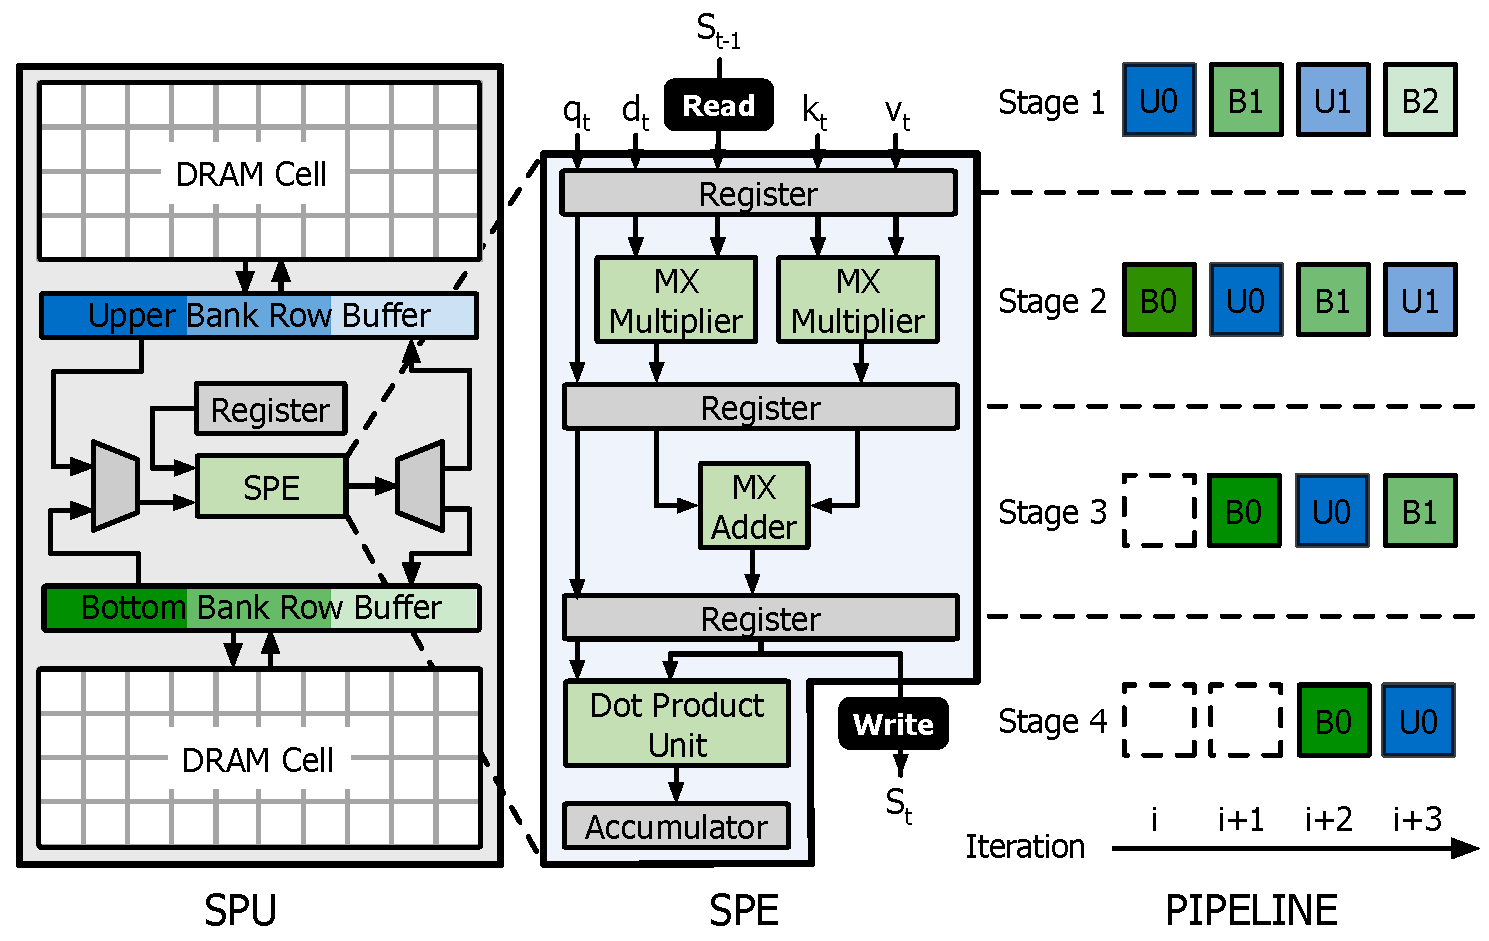
\includegraphics[width=0.95\linewidth]{fig/Pimba_arch.pdf}
  \caption{\sysname{} accelerator architecture leveraging access interleaving.}
  \label{fig:Pimba_arch}
\end{figure}
%

%
\niparagraph{(3) PIM banks with state data layout.}
%
We divide each state column along the $dim_{head}$ dimension into
sub-chunks based on the DRAM column size.
%
Then, we group sub-chunks across the $dim_{state}$ dimension to form
a chunk that aligns with the DRAM row size, enabling efficient
sequential access within each SPU.
%
To further maximize operand reuse across chunks, we organize the
chunks into chunk groups and assign each group to a DRAM bank.
%
Chunks within the same group share the operands $d_t$, $q_t$, and
$k_t$, and are placed in consecutive rows of the bank.
%
This arrangement enables the transfer of shared operands to \sysname{}
once per chunk group, while only the corresponding $v_t$ vector is
transferred per chunk, enhancing data reuse.
%
Once assigned to banks, \sysname{} processes sub-chunks sequentially in
a pipelined manner by reading consecutive columns within a DRAM row.
%
In the $i$-th iteration (time unit during which \sysname{} processes
each sub-chunk), \sysname{} utilizes the $i$-th sub-chunk, the shared
$d_t$, $q_t$, $k_t$ vectors, and the $i$-th element of the $v_t$
vector in its computations.
%

\subsection{Hazard-Free SPU with Access Interleaving}
\label{subsec:access_interleaved_iteration_parallelism}
%
We propose the access interleaving technique, which maintains the
same throughput as per-bank pipelined designs and reduces area overhead by half.
%
The core idea, as illustrated in Figure~\ref{fig:Pimba_arch}, is to
have two memory banks share a single SPU, which alternates between
banks in each iteration, enabling continuous data flow by solving the
structural hazard.
%
At a given iteration, SPU reads a sub-chunk from one bank, referred
to as the upper bank, to initiate a new computation.
%
Simultaneously, the other bank, referred to as the bottom bank,
performs a write operation to store the result of a computation
initiated several iterations earlier.
%
This alternating pattern is sustained in the next iteration: the
upper bank now completes a prior computation by writing its result,
while SPU reads a fresh sub-chunk from the bottom bank to begin
another computation.
%

\begin{figure}[t]
  \centering
  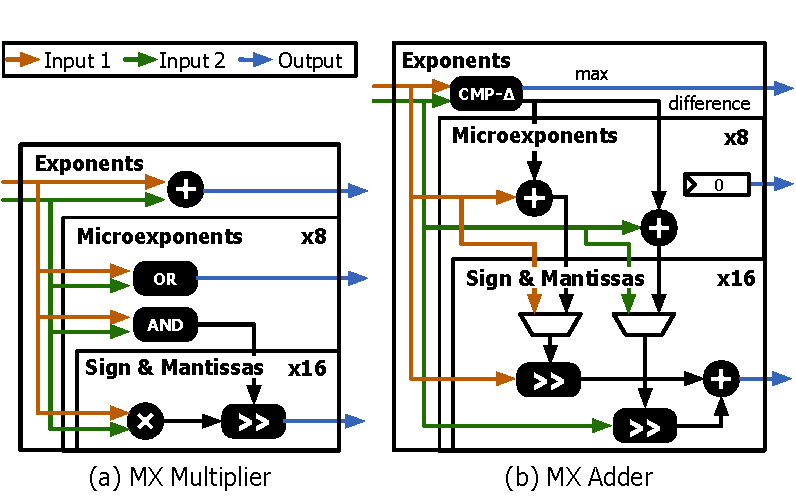
\includegraphics[width=0.9\linewidth]{fig/mx_operation.pdf}
  \caption{Implementation of MX operations in \sysname{} SPE.}
  \label{fig:mx_operation}
\end{figure}

%
\niparagraph{Pipeline.}
%
As depicted in Figure~\ref{fig:Pimba_arch}, \sysname{} employs a
four-stage pipeline:
%
(1): Fetch the state from DRAM.
%
(2): Compute state decay and the outer product in parallel.
%
(3): Sum the results from Stage 2 to update the state.
%
(4): Perform a dot product between the updated state and $q_t$  while
writing the updated state back to DRAM.
%

%
The figure describes the detailed pipelining steps over iteration.
%
Before iteration $i$, operands are loaded into registers, and chunks
in both upper and bottom banks are activated.
%
At iteration $i$, sub-chunk $U0$ from the upper bank is read, while
sub-chunk $B0$ from the bottom bank, which is read in a previous
iteration, enters Stage 2.
%
In iteration $i+1$, sub-chunk $B1$ is read from the bottom bank,
while $U0$ and $B0$ advance to the next stage.
%
At iteration $i+2$, $U1$ is read from the upper bank, and $B0$ is
written back to the bottom bank.
%
Notably, at this point, $U1$ is read from the upper bank while $B0$
is written to the bottom bank, avoiding any conflicts due to the use
of separate banks for read and write operations.
%
Similarly, at iteration $i+3$, $B2$ is read from the bottom bank
while $U0$ is written back to the upper bank.
%
This interleaving allows continuous, conflict-free processing and
ensures full utilization of compute resources, as SPU receives data
every iteration.
%

\subsection{Microarchitecture of MX-based SPE}
\label{subsec:microarchitecture}

%
The MX format, initially designed to accelerate GEMM operations,
requires specific modifications to support element-wise
multiplication and addition.
%
To this end, we design MX Multiplier and MX Adder, specifically
customized for state update computations.
%
Each of these computational units operates at three hierarchical
levels: (1) one unit to handle the shared exponent at the group
level, (2) units to manage the microexponents at the sub-group level,
and (3) integer units for each element’s sign and mantissa.
%

\begin{figure}[t]
  \centering
  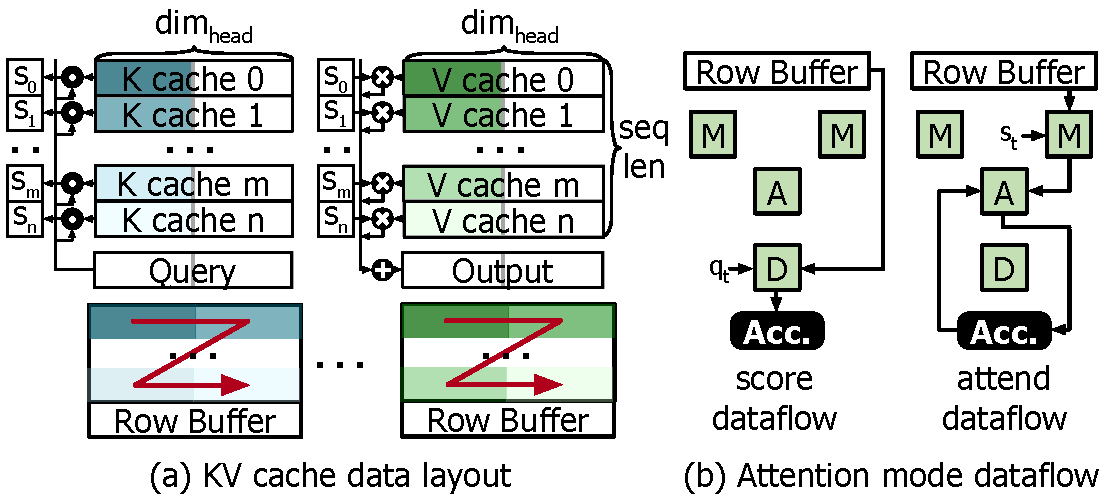
\includegraphics[width=\linewidth]{fig/attention.pdf}
  \caption{(a) KV cache data layout and (b) attention mode dataflow.
    \textit{M} denotes a multipler, \textit{A} an adder, and \textit{D}
  a dot product unit.}
  \label{fig:attention}
\end{figure}

%
\niparagraph{MX multiplier.}
%
Figure~\ref{fig:mx_operation}(a) illustrates how multiplication is
executed with MX.
%
MX Multiplier adds the exponents of the operand groups to compute the
resulting group exponent.
%
Similarly, it sums the microexponents within each sub-group.
%
If the sum of the microexponents exceeds the representable range
(i.e., results in a value of 2, which cannot be represented with 1
bit), it sets the resulting microexponent to 1, and right-shifts the
resulting mantissas of the elements in that sub-group by one, thus
properly adjust the scaling.
%
The sign and mantissa of each element serve as integers, and are
multiplied using integer multiplication units.
%

%
\niparagraph{MX adder.}
%
Figure~\ref{fig:mx_operation}(b) illustrates how addition is executed with MX.
%
Addition in MX necessitates an alignment step to ensure operands are
scaled correctly.
%
MX Adder first aligns the exponents by comparing the two operand
exponents to get their max, which is then used as the resulting exponent.
%
The group with the smaller exponent adjusts its mantissas by
right-shifting them based on the difference between the exponents.
%
Additionally, MX Adder further right-shifts the mantissas by their
respective microexponents to ensure proper alignment.
%
It, then, adds sign and mantissa of each element using integer addition units.
%
The result of the addition operation always produces a micro-exponent of 0.

%
\begin{figure}[t]
  \centering
  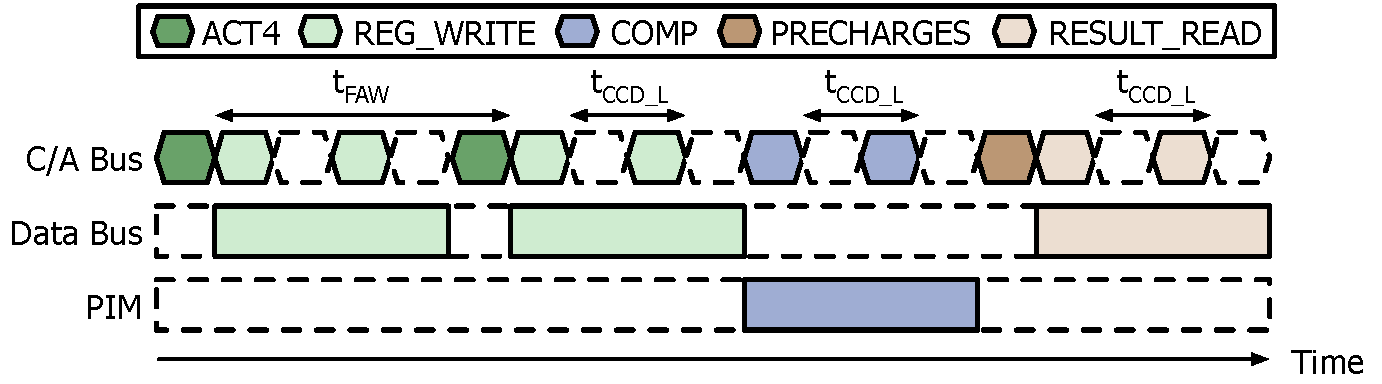
\includegraphics[width=\linewidth]{fig/command_scheduling.pdf}
  \caption{\sysname{} command scheduling. For simplicity, we align C/A
  bus, data bus, and PIM.}
  \label{fig:command_scheduling}
\end{figure}

\subsection{Attention Support in \sysname{}}
\label{subsec:attention_support}
%
Having described how \sysname{} accelerates state update operations, we
now describe its support for attention operations.
%
Notably, \sysname{} reuses its existing logic to efficiently execute
attention operations without requiring dedicated hardware extensions.
%
Figure~\ref{fig:attention}(a) illustrates the layout of the key-value
(KV) cache for attention in \sysname{}.
%
Similar to the state update data layout, we partition each KV cache
along the $dim_{head}$ dimension into sub-chunks sized to match the
DRAM column width.
%
These sub-chunks are then grouped into chunks and mapped contiguously
within DRAM rows, preserving spatial locality and reducing access overhead.
%

%
The attention computation in \sysname{} proceeds in two phases: score
and attend.
%
In the score phase, \sysname{} performs dot products between the query
vector and key vectors using its in-pipeline dot product unit as
shown in the score dataflow of Figure~\ref{fig:attention}(b).
%
The intermediate results are sent to the GPU, where they are
accumulated and passed through a softmax function to produce
normalized attention scores.
%
In the attend phase, \sysname{} multiplies each attention score with
its corresponding value vector and accumulates the results.
%
This phase utilizes \sysname{}'s multiplier and adder units, as shown
in the attend dataflow of Figure~\ref{fig:attention}(b).
%
By leveraging a shared microarchitectural substrate, \sysname{}
achieves efficient support for both state update and attention
operations, demonstrating the versatility of its PIM-based execution model.
%

\subsection{Memory Interface}
\label{subsec:memory_interface}
%
In designing \sysname{}, we extend the standard DRAM interface to
enable practical PIM deployment for SU-LLMs.
%
To achieve this, \sysname{}
%
(1) adheres to existing DRAM timing constraints to reduce engineering
complexity,
%
(2) ensures operations perform predefined functions, aligning with
DRAM refresh schemes,
%
(3) extends the existing DRAM commands to maintain compatibility with
current DRAM, and
%
(4) employs an all-bank design, as in prior PIMs~\cite{newton,
hbm_pim, gradpim}, to minimize logic overhead.
%
We propose five custom DRAM commands for state update and attention operations.
%

%
\begin{itemize}[leftmargin=*]
    %
  \item{\textbf{ACT4.}}
    %
    The portion of the state and KV cache being processed must first
    be activated to the row buffer.
    %
    Due to power constraints and the $t_{FAW}$ timing window for four
    activations, \sysname{} gangs four activations together, similar to
    previous PIMs~\cite{newton, heo2024neupims}.
    %
  \item{\textbf{REG\_WRITE.}}
    %
    Before operations, \sysname{} receives operands from the host in
    \texttt{MX8} format and stores them in the registers using
    REG\_WRITE command.
    %
    If the host lacks \texttt{MX8} support, Quantization Unit can be
    employed in the host’s memory controller, which can be
    implemented by determining the maximum exponent of incoming
    values and adjusting their mantissas using shift operations,
    enabling a very small area implementation.
    %
  \item{\textbf{COMP.}}
    %
    With states activated and operands loaded, the host initiates
    state update/attention operations across all banks using the COMP command.
    %
    Given that each column read occupies I/O gating, consecutive COMP
    commands must observe the $t_{CCD\_L}$ timing constraint~\cite{gradpim}.
    %
  \item{\textbf{RESULT\_READ.}}
    %
    After computations, the host retrieves results using the
    RESULT\_READ command.
    %
    Since COMP involves both reads and writes for state update
    operations, RESULT\_READ must follow COMP with $t_{RTP}$ and
    $t_{WR}$ intervals.
    %
  \item{\textbf{PRECHARGES.}}
    %
    Through state update operations, the row buffer of each bank
    contains updated state values.
    %
    To store these back into DRAM cells and for the next operations,
    all banks' row buffers are precharged using the PRECHARGES command.
    %
\end{itemize}

%
\niparagraph{Command scheduling.}
%
Transferring operands and retrieving results introduce significant
overhead, even with operand reuse.
%
To reduce this overhead, \sysname{} overlaps data transfer between the
host and \sysname{} during activation and precharge, minimizing this
overhead, as depicted in Figure~\ref{fig:command_scheduling}.
%
Specifically, the REG\_WRITE command is inserted into the idle time
between ACT4 commands due to the $t_{FAW}$ timing constraint.
%
Similarly, PRECHARGES takes $t_{RP}$ time to complete, during which
RESULT\_READ is overlapped to reduce the overhead caused by data transmission.
%

\subsection{Intra- and Inter-\sysname{} Communication}
\label{subsec:interaction}
%
\niparagraph{Intra-\sysname{} communication.}
%
\sysname{} attaches the PIM directly to the GPU's off-chip memory,
minimizing communication overhead.
%
Furthermore, all custom commands executed by \sysname{} operate with
deterministic timing, allowing the GPU to issue multiple PIM
commands in sequence without requiring complex synchronization
logic, as long as timing constraints are satisfied.
%
Once all PIM operations are completed, the GPU retrieves the
results via a RESULT\_READ command, which delivers the computed
values to the host's execution units through the load queue.
%
Note that due to data dependencies, GPU and PIM operate in a blocked manner.
%
For instance, in the attention operation, the GPU remains blocked
until \sysname{} completes all score computations.
%
Once completed, the results are transferred to the GPU for the
softmax operation, after which \sysname{} resumes to perform the
attend computation.

\begingroup
\begin{table}[t]
  \small
  \caption{Specifications of the evaluated HBM.}
  \label{tab:specs}
  \begin{center}
    \begin{tabular}{cc}
      % HBM Organization
      \toprule
      \multicolumn{2}{c}{\textbf{HBM Organization}} \\
      \midrule
      Banks/Bank group & 4 \\
      \midrule
      Bank groups/Pseudo-channel & 4 \\
      \midrule
      Memory Bus Frequency & 1.512GHz \\
      \midrule
      PIM Frequency & {378MHz} \\

      % HBM Timing Parameters
      \midrule
      \multicolumn{2}{c}{\textbf{HBM Timing Parameters}} \\
      \midrule
      \multicolumn{2}{c}{tRP = 14, tRAS = 34, tCCD\_S = 2, tCCD\_L =
      4, tWR = 16} \\
      \multicolumn{2}{c}{tRTP\_S = 4, tRTP\_L = 6, tREFI = 3900, tFAW = 30} \\
      \bottomrule
    \end{tabular}
  \end{center}
\end{table}
\endgroup

%
\begin{figure*}[ht]
  \centering
  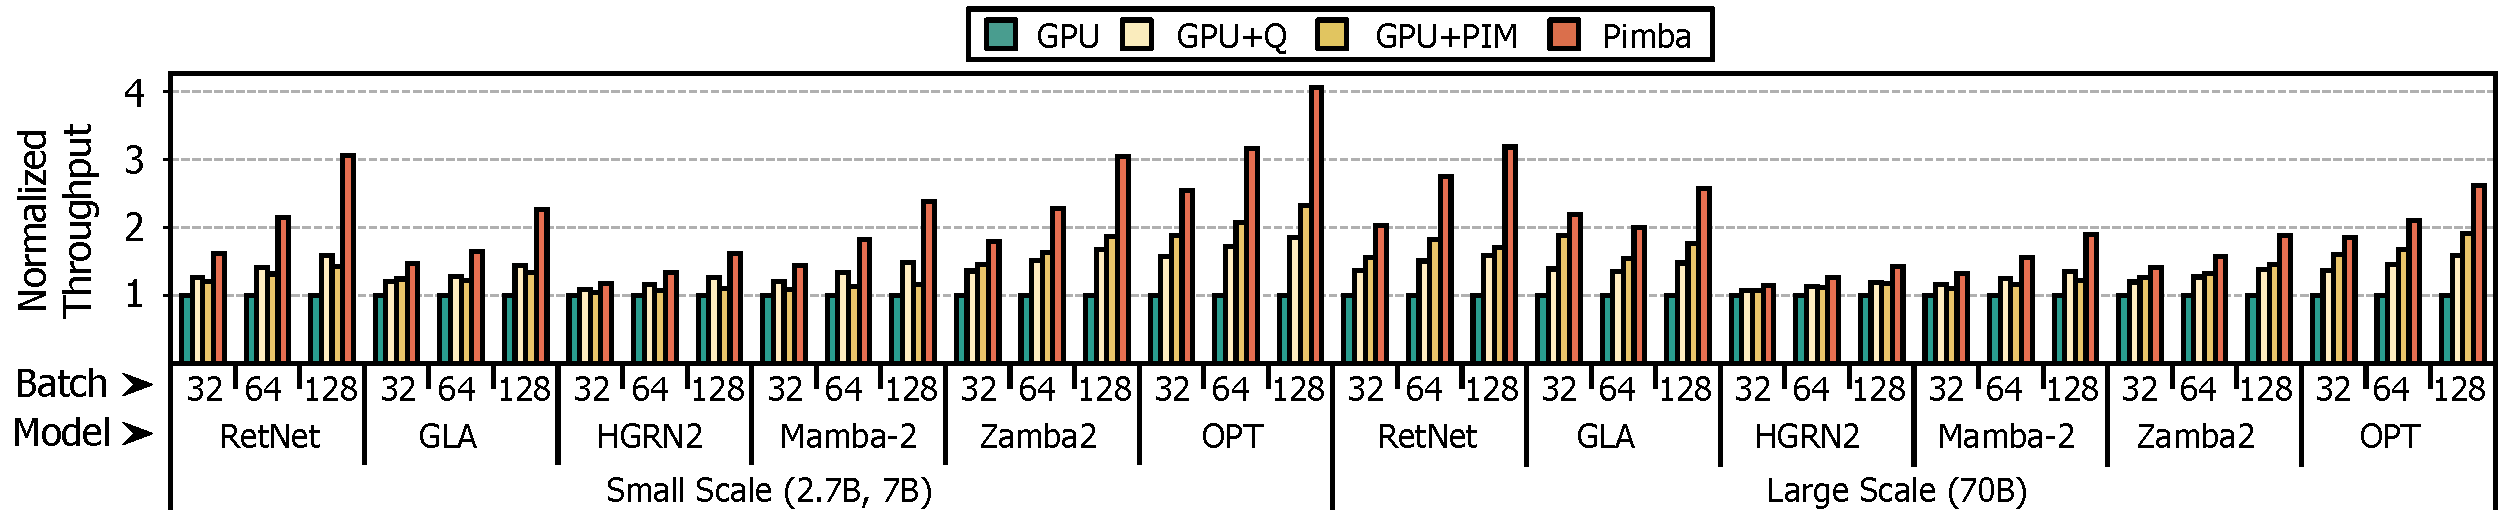
\includegraphics[width=0.95\linewidth]{fig/performance_end_to_end.pdf}
  \caption{Normalized generation throughput on the baselines and
  \sysname{} on various SU-LLMs and an attention-based LLM.}
  \label{fig:performance_end_to_end}
\end{figure*}
%
\begin{figure*}[t]
  \centering
  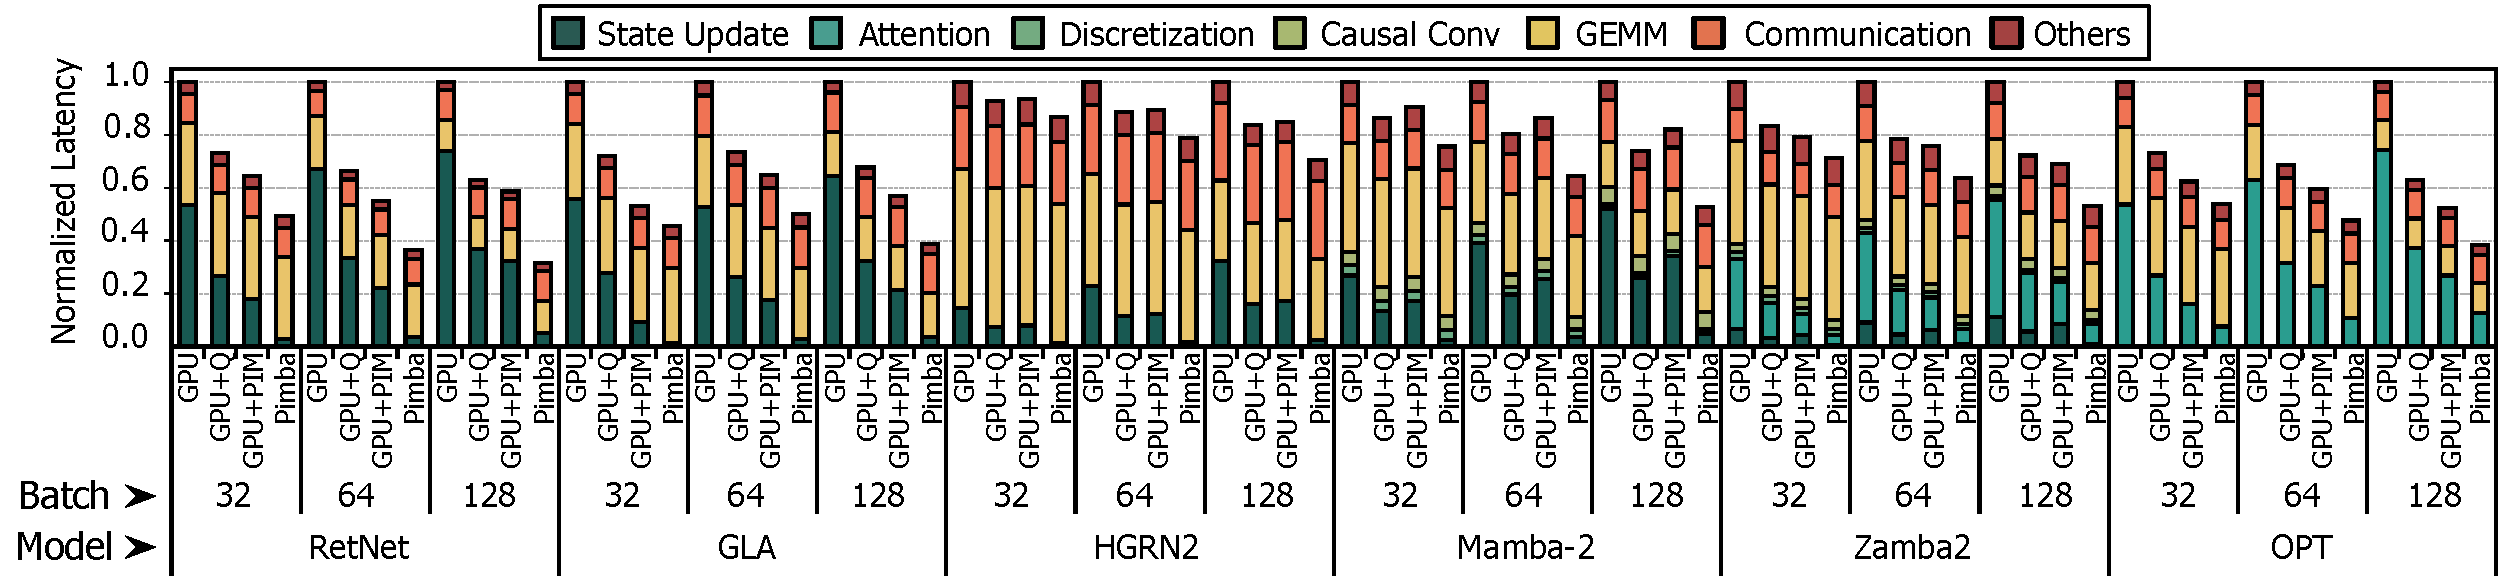
\includegraphics[width=\linewidth]{fig/performance_generation.pdf}
  \caption{Latency breakdown of large scale SU-LLMs and an
    attention-based LLM at generation phase with (2,048, 2,048)
  input/output sequence lengths.}
  \label{fig:performance_generation}
\end{figure*}
%

%
\niparagraph{Inter-\sysname{} communication.}
%
As LLMs continue to grow in size, a single \sysname{} device cannot
support large-scale models.
%
\sysname{} addresses this problem by leveraging pipeline and tensor
parallelism, which distributes the model parameters across multiple devices.
%
To enable such model parallelism, \sysname{} devices exchange
intermediate results via high-bandwidth interconnects such as NVLink.
%
With pipeline parallelism, the model is partitioned into sequential
blocks, each assigned to a different device, and intermediate
results are forwarded to the next \sysname{} device at block boundaries.
%
With tensor parallelism, the QKVD projection layers are sharded
along the output channel dimension, and each device computes
partial QKVD vectors.
%
As state update and attention operate per head, each device
processes only the heads corresponding to its partial vectors.
%
The outputs are then projected using projection matrices sharded
along the input dimension and aggregated across devices via an
all-reduce operation.
%
A similar all-reduce is performed after the FFN to complete the
block’s computation.
%
